% Uncomment the next line for a flat handout PDF (no build duplicates):
%\documentclass[aspectratio=169,10pt,handout]{beamer}
% Comment the next line when using handout mode:
\documentclass[aspectratio=169,10pt]{beamer}

\usetheme{metropolis}
\usepackage{appendixnumberbeamer}
\usepackage{booktabs}
\usepackage{amsmath,amssymb}
\usepackage{tikz}
\usetikzlibrary{arrows.meta,positioning,calc,decorations.pathreplacing,shapes.geometric,fit}
\usepackage{pgfplots}
\pgfplotsset{compat=1.18}
\usepackage{xcolor}
\usepackage{multicol}
\usepackage{graphicx}
\usepackage{hyperref}
\hypersetup{colorlinks=true,urlcolor=columbia,linkcolor=columbia}

% Columbia-inspired palette
\definecolor{columbia}{RGB}{29,79,145}
\definecolor{columbialight}{RGB}{117,170,219}
\definecolor{columbiaaccent}{RGB}{210,73,42}
\definecolor{columbiagray}{RGB}{117,117,117}
\definecolor{softbg}{RGB}{245,245,250}
\definecolor{hlgreen}{RGB}{46,139,87}

\setbeamercolor{frametitle}{bg=columbia,fg=white}
\setbeamercolor{progress bar}{fg=columbiaaccent}
\setbeamercolor{alerted text}{fg=columbiaaccent}
\setbeamercolor{block title}{bg=columbia,fg=white}
\setbeamercolor{block body}{bg=softbg}

\setbeamerfont{title}{size=\Large,series=\bfseries}
\setbeamerfont{subtitle}{size=\normalsize}

\graphicspath{{./figures/}}

\title{Lecture 25: DNA, Genetics \& Gene Regulation}
\subtitle{BINF 4002 --- Machine Learning for Health}
\author{Matthew McDermott}
\institute{Dept.\ of Biomedical Informatics, Columbia University}
\date{April 21, 2026}

\begin{document}

% ============================================================
\begin{frame}[noframenumbering]
\maketitle
\end{frame}

% ============================================================
\begin{frame}{Where We Are}
\textbf{Modality progression:}
\begin{itemize}
    \item[\textcolor{columbiagray}{$\bullet$}] L17--18: EHR \& Claims \quad\textcolor{columbiagray}{$\bullet$} L19--20: Clinical Text \& NLP
    \item[\textcolor{columbiagray}{$\bullet$}] L21--22: Clinical Imaging \quad\textcolor{columbiagray}{$\bullet$} L23: Population Health \quad\textcolor{columbiagray}{$\bullet$} L24: Fairness
    \item[\textcolor{columbiaaccent}{$\to$}] \alert{L25: DNA, Genetics \& Gene Regulation} $\gets$ \textbf{today}
    \item[\textcolor{columbiagray}{$\circ$}] L26: Proteins, Molecules \& Structural Biology
    \item[\textcolor{columbiagray}{$\circ$}] L27: Modern Biological AI
\end{itemize}

\vspace{0.3em}
\textbf{Three lectures on molecular/biological data:}
\begin{enumerate}[<+->]
    \item \textbf{Today:} The genome --- DNA, genetic variation, association analysis, gene regulation
    \item \textbf{L26:} The molecular level --- proteins, small molecules, classical analysis methods
    \item \textbf{L27:} What deep learning adds --- and where it fails
\end{enumerate}
\end{frame}

% ============================================================
\begin{frame}{Learning Objectives}
By the end of today you should be able to:
\begin{enumerate}[<+->]
    \item \textbf{Describe} the central dogma and why DNA alone is insufficient to predict phenotype
    \item \textbf{Explain} what genetic variants are and how they're measured
    \item \textbf{Identify} population structure as the dominant signal in genetic data --- and a confounder
    \item \textbf{Describe} GWAS: univariate testing, effect sizes, multiple testing correction
    \item \textbf{Interpret} Manhattan plots, QQ plots, and genomic inflation factor $\lambda$
    \item \textbf{Define} PRS and explain the cross-ancestry transferability problem
    \item \textbf{Explain} how gene expression connects genotype to phenotype, and why context matters
\end{enumerate}
\end{frame}


% ============================================================
\section{DNA and the Central Dogma}
% ============================================================

% ============================================================
\begin{frame}{The Central Dogma}
\begin{center}
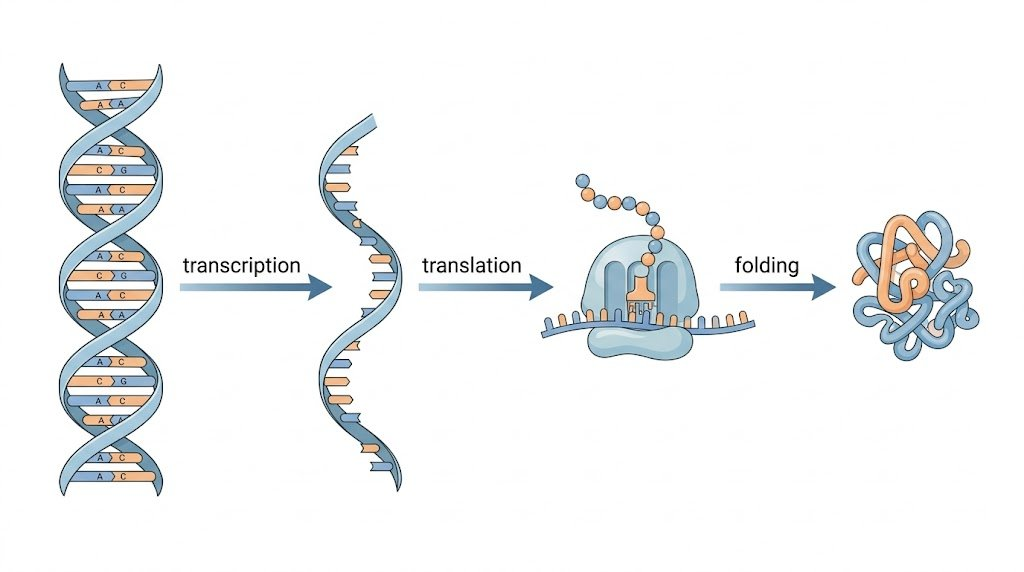
\includegraphics[width=0.95\textwidth,height=0.68\textheight,keepaspectratio]{fig25_central_dogma.png}
\end{center}
\vspace{-0.3em}
{\small Each arrow is a place where ML can help: variant effect prediction, expression prediction, structure prediction, function prediction. Today we focus on the first step: DNA and genetic variation.}
\end{frame}

% ============================================================
\begin{frame}{DNA Basics}
\textbf{Four bases:} A, T, G, C. Double helix with complementary base pairing (A-T, G-C).

\vspace{0.2em}
\textbf{Scale:} 3.2 billion base pairs, 23 chromosome pairs, ${\sim}20{,}000$ protein-coding genes --- but protein-coding exons are only ${\sim}1$--$2\%$ of the genome. Most DNA is noncoding; some is regulatory, and much remains incompletely characterized.

\vspace{0.2em}
\textbf{The genome as a reference:} We have a ``reference genome'' (GRCh38). Individual variation is measured \emph{relative to} this reference.

\vspace{0.2em}
{\footnotesize
\begin{center}
\begin{tabular}{ll}
\toprule
\textbf{What we have} & \textbf{Scale} \\
\midrule
Human genomes genotyped (arrays) & $>$1 million (e.g., UK Biobank, 23andMe) \\
Whole-genome sequences (WGS) & ${\sim}76{,}000$ (gnomAD v4) \\
Exome sequences (WES) & ${\sim}730{,}000$ (gnomAD v4) \\
Protein-coding genes identified & ${\sim}20{,}000$ \\
Variant--disease associations (GWAS Catalog) & ${\sim}400{,}000$ \\
Variants with functional characterization & Much less \\
\bottomrule
\end{tabular}
\end{center}}
\end{frame}

% ============================================================
\begin{frame}{DNA at Three Scales}
\begin{center}
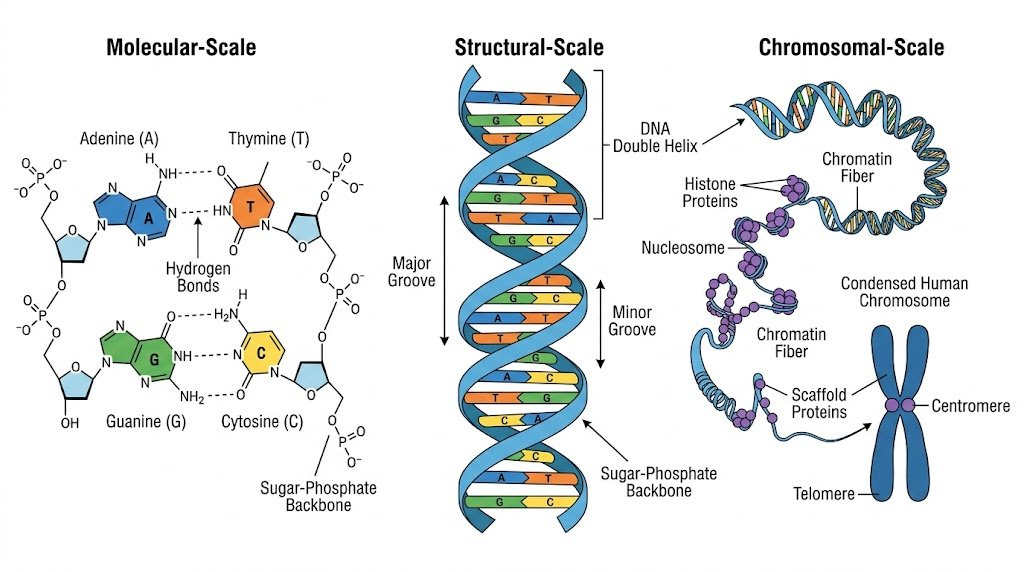
\includegraphics[width=0.95\textwidth,height=0.63\textheight,keepaspectratio]{fig25_dna_structure.png}
\end{center}
\vspace{-0.3em}
{\footnotesize \textbf{Left:} Base pairing chemistry (A-T, G-C) on the sugar-phosphate backbone. \textbf{Center:} The double helix with major/minor grooves (where proteins bind to regulate gene expression). \textbf{Right:} DNA wraps around histones $\to$ chromatin fiber $\to$ condensed chromosome. Packaging affects which genes are accessible.}
\end{frame}

% ============================================================
\begin{frame}{Genetic Variants}
\textbf{SNPs} (single nucleotide polymorphisms): one base differs from reference. The most common variant type (${\sim}4$--$5$M per individual).

\vspace{0.2em}
Other types: insertions/deletions (indels), structural variants (large rearrangements). Today: SNPs --- the workhorse of genetic association studies.

\vspace{0.2em}
\textbf{Minor allele frequency (MAF):} Common ($>1\%$, well-tagged by arrays) vs.\ rare ($<1\%$, require sequencing).

\vspace{0.3em}
\textbf{The genotype matrix:} $n$ individuals $\times$ $p$ SNPs. Each entry $\in \{0,1,2\}$ = copies of alternate allele.

\vspace{0.2em}
\begin{block}{Data Type Box}
\textbf{TABULAR}, but $p \gg n$ (${\sim}5$M SNPs, ${\sim}10^3$--$10^6$ individuals), with structured correlation (LD) and population stratification as dominant confounder.
\end{block}
\end{frame}

% ============================================================
\begin{frame}{Measuring Genetic Variation}
\begin{columns}[T]
\column{0.32\textwidth}
\textbf{SNP Arrays}
\begin{center}
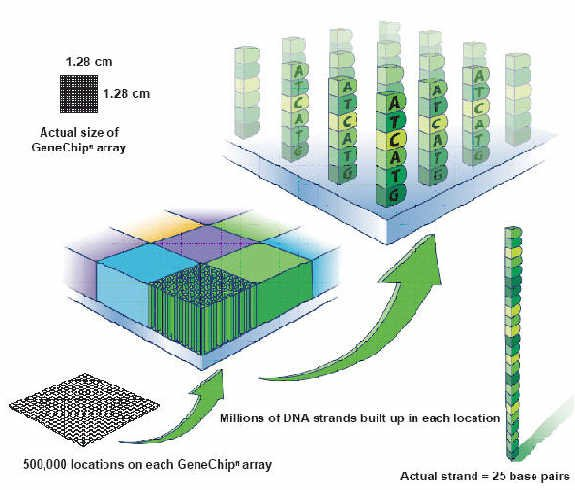
\includegraphics[width=0.85\textwidth,height=0.25\textheight,keepaspectratio]{fig25_snp_array.png}
\end{center}
\vspace{-0.3em}
{\footnotesize Targeted: ${\sim}500$K--$5$M pre-selected SNPs. Cheap (${\sim}\$50$--$\$200$). Most large GWAS use arrays + imputation. Miss rare variants entirely.}

\column{0.32\textwidth}
\textbf{Exome Sequencing (WES)}
\vspace{0.2em}

{\footnotesize Sequences protein-coding regions (${\sim}2\%$ of genome). Better coding coverage than arrays, better depth than WGS. Moderate cost (${\sim}\$100$--$\$400$). Widely used in clinical diagnostics and large cohorts (gnomAD: ${\sim}730$K exomes). Misses noncoding regulatory variants.}

\column{0.32\textwidth}
\textbf{Whole-Genome Seq.}
\begin{center}
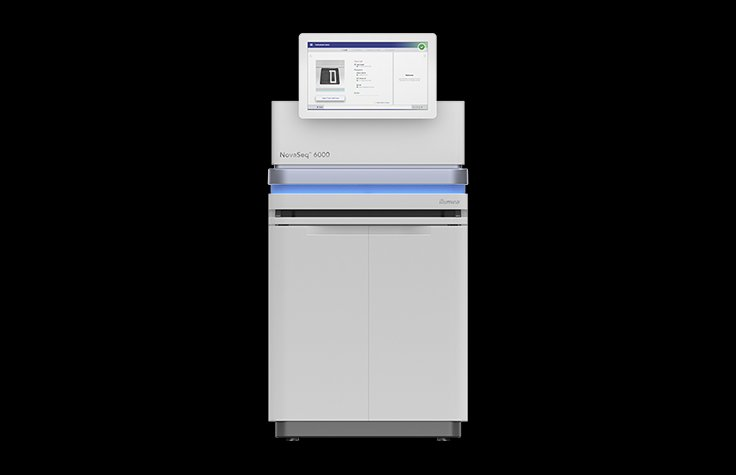
\includegraphics[width=0.85\textwidth,height=0.25\textheight,keepaspectratio]{fig25_novaseq.png}
\end{center}
\vspace{-0.3em}
{\footnotesize Comprehensive: all 3.2B positions. More expensive (${\sim}\$200$--$\$1{,}000$). Detects rare variants, noncoding, SVs. Growing but still smaller cohorts (gnomAD: ${\sim}76$K WGS).}
\end{columns}

\vspace{0.2em}
{\footnotesize \textbf{Clinical applications:} BRCA1/2 testing, pharmacogenomics, carrier screening.
\textbf{Key databases:} gnomAD, ClinVar, GWAS Catalog, 1000 Genomes.}
\end{frame}


% ============================================================
\section{Population Structure}
% ============================================================

% ============================================================
\begin{frame}{Genes Mirror Geography}
\begin{center}
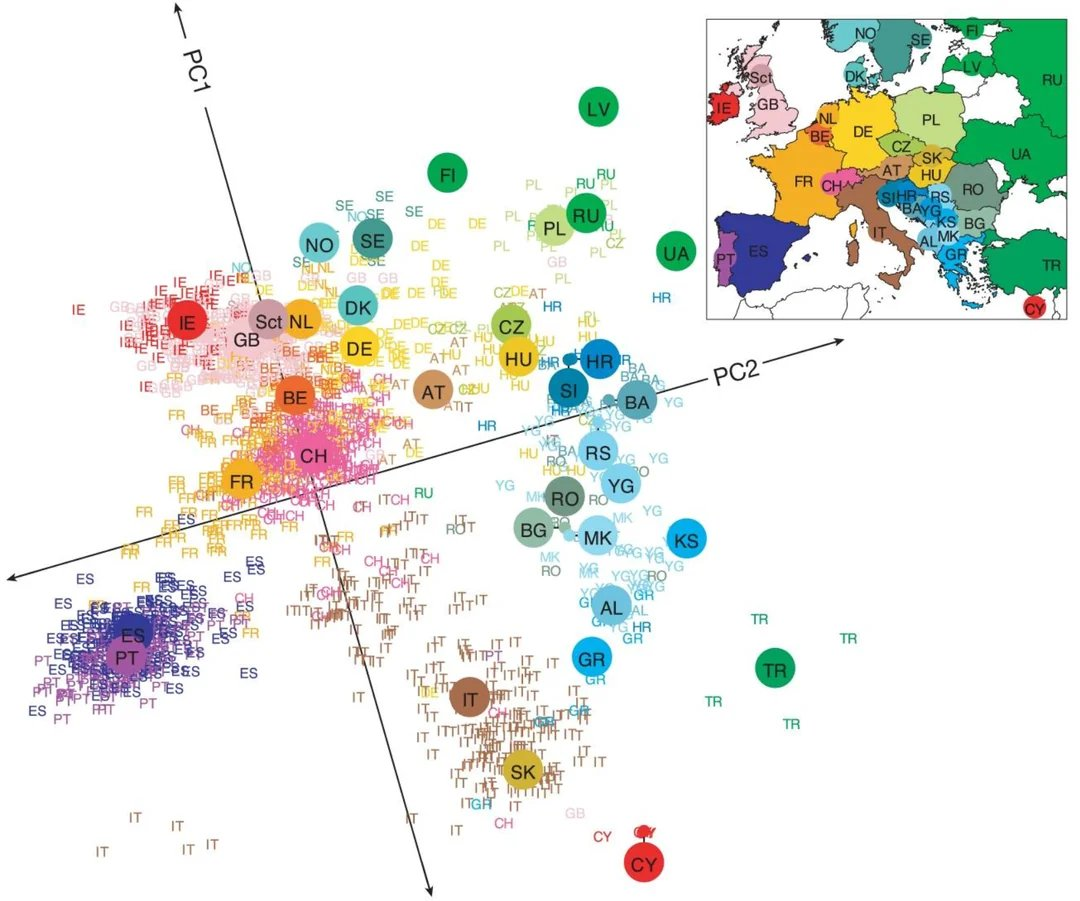
\includegraphics[width=0.85\textwidth,height=0.64\textheight,keepaspectratio]{fig25_pca_europe.png}
\end{center}
\vspace{-0.5em}
{\footnotesize Novembre et al., \textit{Nature} 2008. PCA of ${\sim}200$K SNPs from ${\sim}1{,}400$ Europeans recovers the map of Europe. Each point is a person; position is determined entirely by genetics. \textbf{The dominant signal in genetic data is ancestry, not disease.}}
\end{frame}

% ============================================================
\begin{frame}{Why This Is a Problem for ML}
\textbf{You just saw:} PCA on genetic data recovers geography. Human migration history imprinted allele-frequency differences across populations over thousands of generations.

\vspace{0.3em}
\textbf{Disease effects} are tiny: common-variant per-allele effects usually have odds ratios around 1.01--1.2. Collectively, thousands of such variants explain 5--50\% of trait variance.

\vspace{0.3em}
\begin{block}{Consequence for ML}
A naive classifier on raw genotype features will learn \emph{ancestry} and call it ``disease risk.'' Any ancestry group with higher prevalence (even from socioeconomic factors) gets flagged as high-risk.
\end{block}

\vspace{0.2em}
\textbf{Connection to L17:} An extreme $p \gg n$ problem. With ${\sim}5$M features and ${\sim}5$K samples, overfitting to population structure is the default.
\end{frame}

% ============================================================
\begin{frame}{Linkage Disequilibrium (LD)}
\textbf{LD:} Nearby variants on the same chromosome are co-inherited. They are \emph{not} independent features.

\vspace{0.3em}
\textbf{Consequences for ML:}
\begin{enumerate}[<+->]
    \item A significant GWAS hit may not be the causal variant --- it could be a correlated neighbor
    \item Feature selection methods that assume independence find clusters of hits, not single causal variants
    \item Regularized models (LASSO) can arbitrarily choose one SNP from an LD block
\end{enumerate}

\vspace{0.3em}
\textbf{Analogy:} LD is to genetics what multicollinearity is to regression --- correlated features where the model can't distinguish cause from proxy.
\end{frame}


% ============================================================
\section{GWAS}
% ============================================================

% ============================================================
\begin{frame}{Genome-Wide Association Study: The Approach}
\textbf{Goal:} Find SNPs \emph{associated} with a trait (disease status, biomarker, etc.)

\textbf{Method:} Test each SNP \emph{independently} ($\chi^2$ or logistic regression for binary traits; linear regression for continuous).

\vspace{0.2em}
\alert{Key distinction from ML:} GWAS asks ``is $\hat{\beta}$ significantly non-zero?'' --- not ``does this SNP improve prediction?'' We identify \emph{which} variants matter, not build the best classifier.

\vspace{0.1em}
{\small \textbf{Why not a multivariate model?} $p \gg n$: can't fit $5$M coefficients with $5$K samples. Each SNP has a tiny effect ($\text{OR} \approx 1.01$--$1.2$). GWAS is \emph{feature screening}, not prediction.}

{\footnotesize \textbf{Generalizes beyond disease:} Replace the trait with gene expression $\to$ eQTL; chromatin accessibility $\to$ caQTL. Same framework, different response.}
\end{frame}

% ============================================================
\begin{frame}{Effect Sizes: What ``Significant'' Means}
\textbf{GWAS reports effect sizes} ($\hat{\beta}$ or odds ratio), not prediction accuracy.

\vspace{0.2em}
\begin{itemize}[<+->]
    \item Typical genome-wide significant SNP: $\text{OR} \approx 1.05$--$1.2$, occasionally larger for specific traits
    \item A SNP can reach $p = 10^{-15}$ (extremely significant) and still be \alert{clinically useless} for individual prediction
    \item Significance tells you a variant is \emph{associated}; it says nothing about how well you can \emph{predict} the trait
\end{itemize}

\vspace{0.3em}
\textbf{Why small effects matter:} Disease is polygenic --- thousands of small effects accumulate. Finding the right 50 SNPs out of 5M is a needle-in-a-haystack problem. Statistical significance is the tool for the search, even when each individual effect is tiny.
\end{frame}

% ============================================================
\begin{frame}{GWAS Success Stories: From Loci to Medicine}
\textbf{GWAS is not just an academic exercise.} Real discoveries have changed clinical practice:

\vspace{0.2em}
\begin{itemize}[<+->]\itemsep0.05em
    \item \textbf{PCSK9 $\to$ cholesterol drugs:} GWAS found PCSK9 variants $\to$ rare loss-of-function mutations showed lower heart attack risk $\to$ FDA-approved antibodies (evolocumab, alirocumab) lower LDL by ${\sim}60\%$.
    \item \textbf{FTO $\to$ obesity biology:} First obesity GWAS hit. Causal mechanism involves a \emph{distal} gene (IRX3) via long-range enhancer --- GWAS hits need functional follow-up.
    \item \textbf{CYP2C9 / VKORC1 $\to$ warfarin dosing:} Variants explain ${\sim}40\%$ of variance in optimal dose. Now in pharmacogenomic dosing guidelines (CPIC).
    \item \textbf{HLA $\to$ autoimmune disease:} Strongest GWAS signals for T1D, RA, and celiac all map to HLA/MHC on chr6 --- pointing to immune mechanisms.
\end{itemize}
\end{frame}

% ============================================================
\begin{frame}{Multiple Testing: 5 Million Hypotheses}
Under the null, p-values $\sim \text{Uniform}(0,1)$. At $\alpha = 0.05$ with $5 \times 10^6$ tests: $250{,}000$ expected false positives.

\vspace{0.1em}
\textbf{Bonferroni:} $\alpha_{\text{genome-wide}} = 0.05 / m$. Convention: $5 \times 10^{-8}$ (${\sim}1$M effective tests).
{\footnotesize BH/FDR is less conservative; standard in eQTL analysis.}

\vspace{-0.1em}
\begin{center}
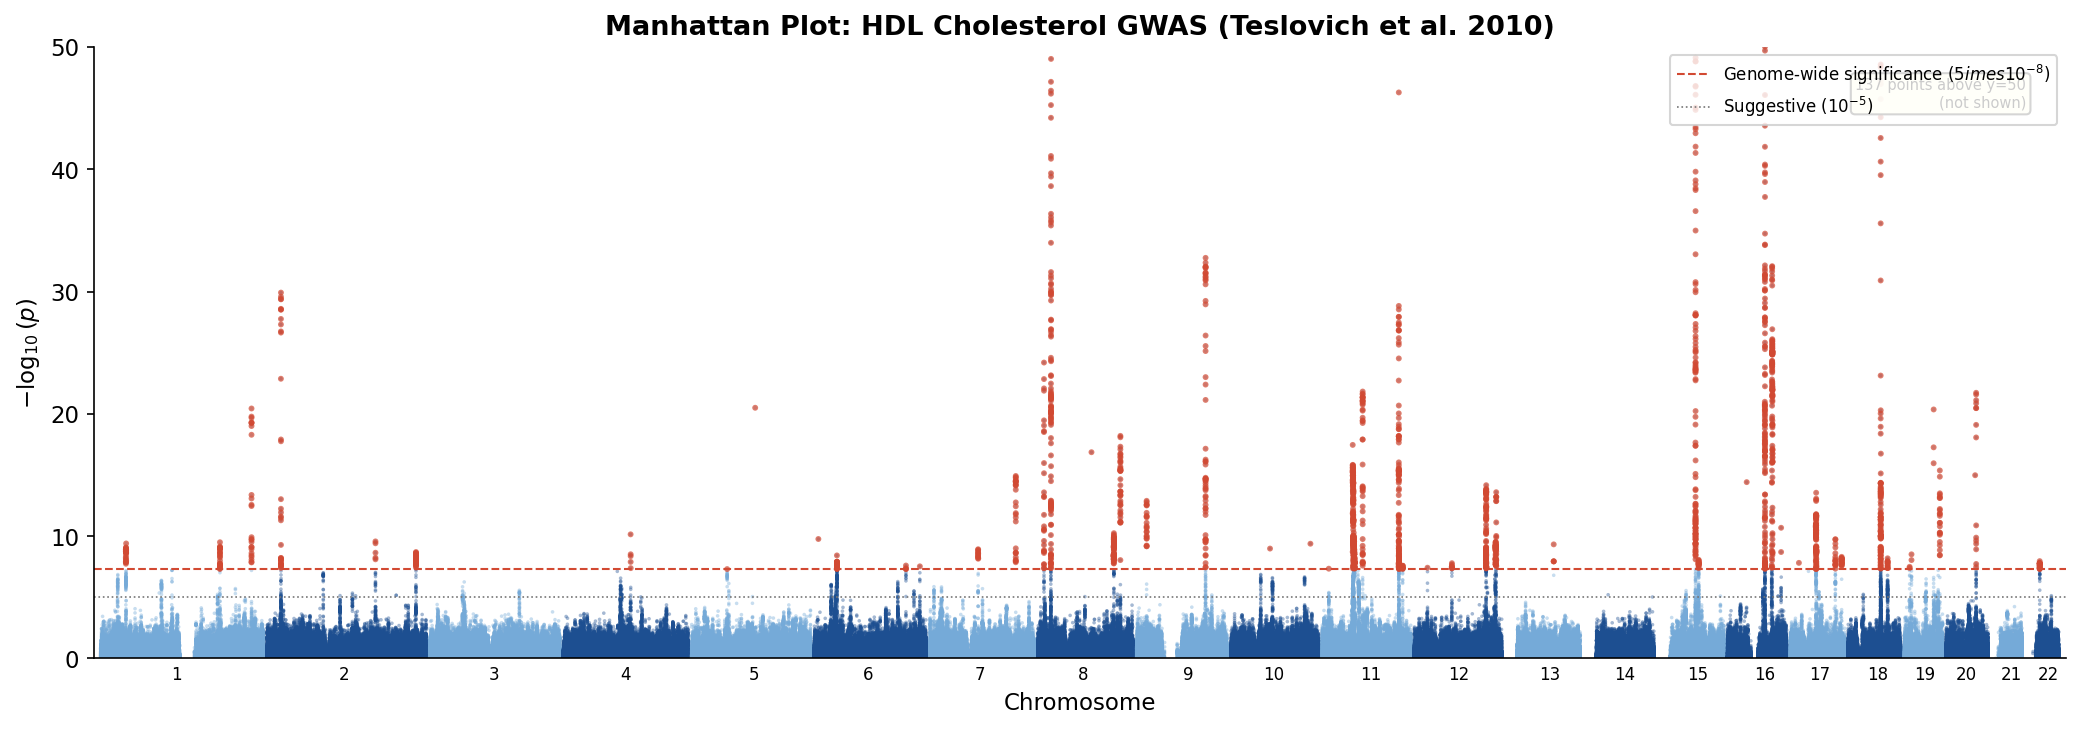
\includegraphics[width=0.95\textwidth,height=0.30\textheight,keepaspectratio]{fig25_1_manhattan.png}
\end{center}
\vspace{-0.5em}
{\footnotesize [Notebook Figure 1] \quad Real GWAS data: HDL cholesterol (Teslovich et al., 2010). Peaks above the red line = genome-wide significant loci.}
\end{frame}

% ============================================================
\begin{frame}{QQ Plot and Genomic Inflation}
\textbf{QQ plot:} Expected vs.\ observed $-\log_{10}(p)$. Since $p \sim \text{Uniform}(0,1)$ under the null, expected quantiles are known. \textbf{Genomic inflation} $\lambda$: median observed $\chi^2$ / 0.456.

\vspace{0.1em}
\begin{columns}[T]
\column{0.45\textwidth}
\begin{center}
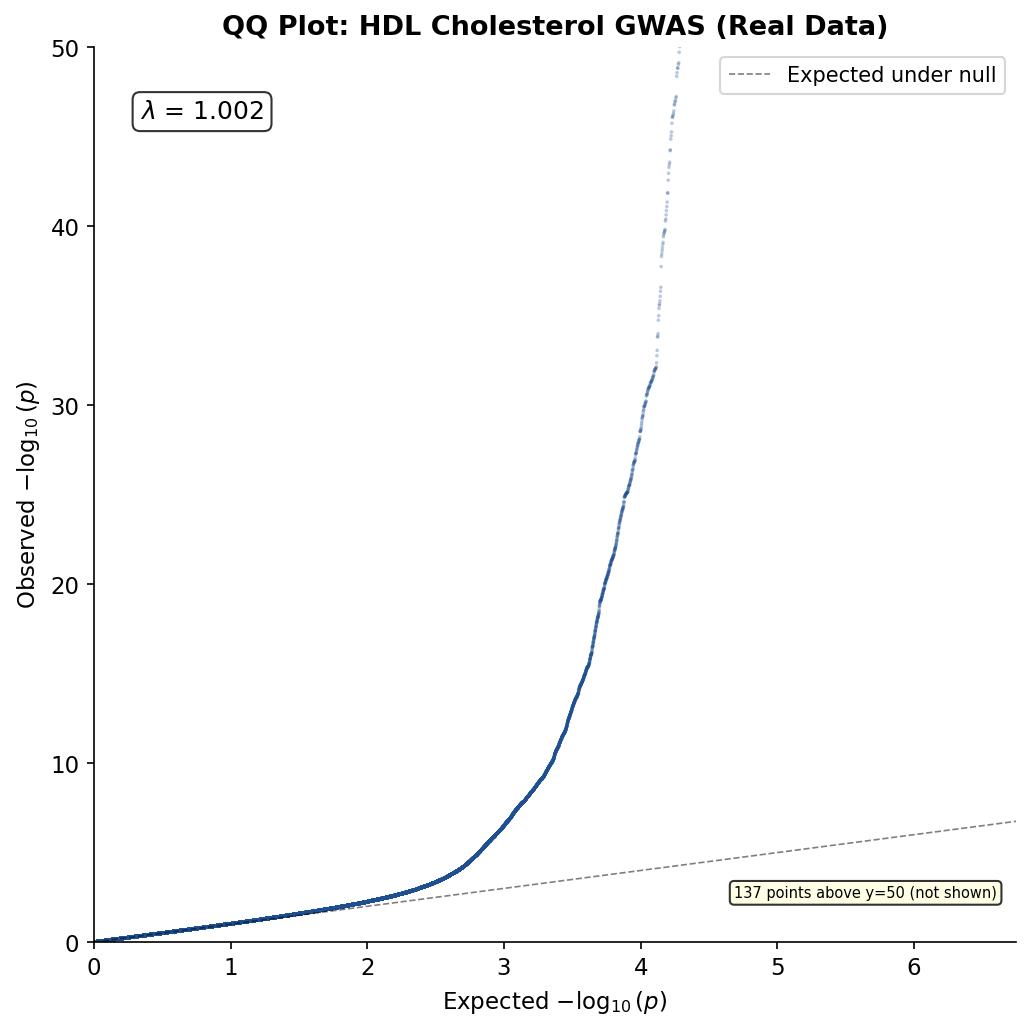
\includegraphics[width=\textwidth,height=0.48\textheight,keepaspectratio]{fig25_2_qq_plot.png}
\end{center}
\vspace{-0.3em}
{\footnotesize [Notebook Figure 2] Real data: HDL cholesterol GWAS.}

\column{0.52\textwidth}
\textbf{Reading the plot:}
\begin{itemize}[<+->]\itemsep0.1em
    \item Bulk follows diagonal $\Rightarrow$ well-calibrated ($\lambda \approx 1$)
    \item Tail lifts off $\Rightarrow$ real associations
    \item If the \emph{whole curve} deviates upward ($\lambda > 1$), suspect confounding or polygenicity
\end{itemize}

\vspace{0.2em}
{\footnotesize $\lambda \approx 1$ is consistent with well-calibrated test statistics. The investigators adjusted for population structure (PCs as covariates). Without adjustment, ancestry-correlated allele frequencies would inflate $\lambda$ genome-wide.}
\end{columns}
\end{frame}

% ============================================================
\begin{frame}{Correcting Population Stratification}
\textbf{Problem:} Population stratification inflates test statistics genome-wide.

\vspace{0.2em}
\textbf{Solution:} Include top PCs of the genotype matrix as covariates:
\[
\text{logit}(P(\text{disease})) = \beta_{\text{SNP}} \cdot g + \sum_{k=1}^{K} \gamma_k \cdot \text{PC}_k
\]

Typically $K = 10$--$20$ PCs. These absorb ancestry signal (recall: PCA recovers the map of Europe), leaving genuine associations.

\vspace{0.1em}
{\small \textbf{Intuition:} If a SNP is associated with disease only because it tracks ancestry, adding PCs absorbs that signal $\to$ non-significant. Genuine causal SNPs remain significant.}

\vspace{0.1em}
\begin{block}{PCs fix stratification, not LD}
{\small If a causal SNP is significant, its LD neighbors will \emph{also} remain significant after PC adjustment --- PCs do not break linkage. LD is addressed separately: clumping/pruning in PRS construction, fine-mapping for causal inference.}
\end{block}
\end{frame}


% ============================================================
\section{Polygenic Risk Scores}
% ============================================================

% ============================================================
\begin{frame}{Polygenic Risk Scores (PRS)}
\textbf{After GWAS:} We have per-SNP effect sizes $\hat{\beta}_i$.

\vspace{0.2em}
\textbf{PRS} for a new individual: $\text{PRS} = \sum_{i=1}^{M} \hat{\beta}_i \times g_i$, \; $g_i \in \{0,1,2\}$.

\vspace{0.2em}
A \textbf{linear model with pre-computed coefficients} --- no fitting on the target sample.

\vspace{0.3em}
\textbf{The construction problem:} GWAS marginal $\hat{\beta}$s are correlated via LD. Naively summing them double-counts shared signal.
\begin{itemize}[<+->]\itemsep0.1em
    \item \textbf{C+T:} Keep most significant SNP per region; prune by $r^2$ threshold. Simple but discards information.
    \item \textbf{Bayesian shrinkage (LDpred, PRS-CS):} Explicitly model LD and regularize $\hat{\beta}$s --- same intuition as ridge regression. Better but more complex.
\end{itemize}
\end{frame}

% ============================================================
\begin{frame}{PRS Transferability and Equity}
${\sim}80\%$ of GWAS participants are of European ancestry.

\vspace{0.3em}
PRS trained on EUR data performs \alert{substantially worse} in non-EUR populations:

\vspace{0.2em}
\begin{center}
{\small
\begin{tabular}{ll}
\toprule
\textbf{Ancestry group} & \textbf{Relative PRS performance} \\
\midrule
European (training population) & 100\% (reference) \\
East Asian & ${\sim}50$--$60\%$ \\
South Asian & ${\sim}40$--$60\%$ \\
African & ${\sim}20$--$40\%$ \\
\bottomrule
\end{tabular}}
\end{center}
\vspace{-0.2em}
{\footnotesize Illustrative summary based on Martin et al., \textit{Nat Genetics} 2019. Performance varies substantially by trait and study design; these are approximate ranges across multiple phenotypes.}

\vspace{0.3em}
\textbf{Why:} LD patterns and allele frequencies differ across ancestries $\Rightarrow$ the ``right'' tag SNP changes. \textbf{Clinical consequence:} EUR-derived PRS systematically underperforms for non-EUR patients. A health equity problem.
\end{frame}


% ============================================================
\section{Gene Expression and Regulation}
% ============================================================

% ============================================================
\begin{frame}{From Genotype to Phenotype: The Missing Middle}
\textbf{GWAS identifies associated SNPs.} But \emph{how} do variants cause disease?

\vspace{0.3em}
\begin{center}
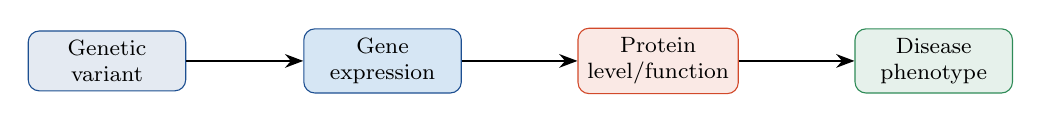
\begin{tikzpicture}[
    box/.style={draw,rounded corners,minimum width=2cm,minimum height=0.6cm,align=center,font=\footnotesize},
    >=Stealth
]
\node[box,fill=columbia!12,draw=columbia] (var) at (0,0) {Genetic\\variant};
\node[box,fill=columbialight!30,draw=columbia] (expr) at (3.5,0) {Gene\\expression};
\node[box,fill=columbiaaccent!12,draw=columbiaaccent] (prot) at (7,0) {Protein\\level/function};
\node[box,fill=hlgreen!12,draw=hlgreen] (pheno) at (10.5,0) {Disease\\phenotype};
\draw[->,thick] (var) -- (expr);
\draw[->,thick] (expr) -- (prot);
\draw[->,thick] (prot) -- (pheno);
\end{tikzpicture}
\end{center}

\vspace{0.3em}
Most GWAS hits are in \emph{non-coding} regions --- they don't change the protein directly. Instead, they alter \textbf{gene regulation}: how much of a gene is transcribed into RNA.

\vspace{0.2em}
{\small \textbf{Example:} The FTO obesity locus doesn't affect FTO itself. The causal variant alters a long-range enhancer that controls IRX3, a gene 500kb away. Regulatory connections can span enormous genomic distances.}
\end{frame}

% ============================================================
\begin{frame}{How Gene Regulation Works}
\textbf{If most GWAS hits are in noncoding regions, what are they disrupting?}

\vspace{0.3em}
\textbf{Regulatory elements} control when, where, and how much a gene is transcribed:
\begin{itemize}[<+->]\itemsep0.1em
    \item \textbf{Promoter:} DNA region just upstream of a gene where RNA polymerase binds to initiate transcription
    \item \textbf{Enhancer:} Distal regulatory element (can be 100kb--1Mb away) that boosts transcription of a target gene when bound by transcription factors (TFs)
    \item \textbf{Chromatin accessibility:} DNA wrapped tightly around histones is inaccessible; regulatory elements must be in ``open chromatin'' to function
\end{itemize}

\vspace{0.2em}
\textbf{Why this matters:} A GWAS-significant SNP in an enhancer may alter TF binding $\to$ change expression of a distal gene $\to$ alter protein levels $\to$ shift disease risk. The variant doesn't change the protein --- it changes \emph{how much} protein is made, and \emph{in which tissues}.
\end{frame}

% ============================================================
\begin{frame}{Gene Expression: RNA as the Intermediate}
\textbf{mRNA} = the intermediate product of the central dogma. Measuring mRNA tells you which genes are ``active'' in a given cell or tissue.

\vspace{0.3em}
\textbf{RNA-seq:} Sequence all mRNA in a sample $\to$ a vector of expression levels across ${\sim}20{,}000$ genes. Each sample = a high-dimensional continuous measurement.

\vspace{0.3em}
\begin{block}{Data Type Box}
\textbf{HIGH-DIMENSIONAL CONTINUOUS.} Genes $\times$ samples matrix (${\sim}20$K $\times$ $n$). For bulk RNA-seq: batch effects, library-size normalization, and the mean-variance relationship are the dominant data quality issues. For single-cell RNA-seq: sparsity and dropout add substantial additional complexity.
\end{block}

\vspace{0.2em}
{\footnotesize \textbf{Key resource:} GTEx v8 (Genotype-Tissue Expression) --- ${\sim}17{,}000$ RNA-seq samples across 54 tissue sites from ${\sim}840$ donors, with matched genotypes. Enables tissue-specific eQTL analysis.}
\end{frame}

% ============================================================
\begin{frame}{eQTL: GWAS for Gene Expression}
\textbf{Same statistical framework as GWAS}, but the response variable is gene expression instead of disease status.

\vspace{0.3em}
\textbf{eQTL} (expression quantitative trait locus): a genetic variant that is statistically associated with the expression level of a gene.

\vspace{0.3em}
\begin{itemize}[<+->]
    \item Test: for each SNP $\times$ gene pair, is $\hat{\beta}$ significantly non-zero?
    \item Scale: genome-wide testing is enormous (${\sim}5$M $\times$ ${\sim}20$K). In practice, most eQTL studies focus on \emph{cis} windows (${\sim}1$Mb around each gene), reducing the burden. FDR/BH correction standard.
    \item Identifies the regulatory \emph{mechanism} behind GWAS hits
\end{itemize}

\vspace{0.3em}
\textbf{Extends to other phenotypes:} caQTL (chromatin accessibility), pQTL (protein levels), sQTL (splicing). Same framework, different molecular readout.
\end{frame}

% ============================================================
\begin{frame}{Why Context Matters: DNA Never Exists in a Vacuum}
\textbf{The same variant can have different eQTL effects} in different tissues, cell types, and developmental stages.

\vspace{0.3em}
A SNP that alters liver gene expression may have \emph{no effect} in the brain --- because the regulatory elements it disrupts are only active in liver.

\vspace{0.3em}
\begin{block}{Implications for modeling}
The \emph{same} DNA in a liver cell and a neuron produces radically different outcomes. Gene regulation is \textbf{context-dependent}. DNA sequence alone does not fully determine expression across tissues, cell states, and environments. This is why DNA foundation models trained on sequence alone (L27) face fundamental limits.
\end{block}
\end{frame}


% ============================================================
\section{Wrap-up}
% ============================================================

% ============================================================
\begin{frame}{Key Databases}
{\small
\begin{center}
\begin{tabular}{lll}
\toprule
\textbf{Database} & \textbf{Content} & \textbf{Use} \\
\midrule
gnomAD & Population allele frequencies & Is this variant common or rare? \\
ClinVar & Variant--disease annotations & Is this variant pathogenic? \\
GWAS Catalog & Published associations & Which SNPs are associated with which traits? \\
GTEx & Expression by tissue + genotype & Tissue-specific eQTL analysis \\
1000 Genomes & Reference genotypes & Population structure, imputation \\
\bottomrule
\end{tabular}
\end{center}}

\vspace{0.3em}
{\small These are the resources your models will train on, validate against, and be compared to. Knowing what each contains --- and what it \emph{doesn't} --- is essential.}
\end{frame}

% ============================================================
\begin{frame}{Key Takeaways}
\begin{enumerate}[<+->]
    \item \textbf{Central dogma has limits:} DNA $\to$ RNA $\to$ protein, but context (tissue, cell type, environment) determines what DNA actually does.
    \item \textbf{Population structure is the dominant signal} in genetic data --- and it's a confounder. Adjust for it or your model learns ancestry, not disease.
    \item \textbf{GWAS = feature screening, not prediction.} Effect size matters; statistical significance $\neq$ clinical utility.
    \item \textbf{But GWAS discoveries have real clinical impact:} PCSK9 inhibitors, pharmacogenomic dosing, and autoimmune disease mechanisms all trace back to GWAS hits.
    \item \textbf{PRS transfers poorly across ancestries} --- a real health equity problem.
    \item \textbf{Context matters.} The same variant has different effects in different tissues --- this limits what sequence-only models can learn.
\end{enumerate}
\end{frame}

% ============================================================
\begin{frame}{Notebook Companion: \texttt{nb25\_dna\_genetics.ipynb}}
{\small Today's notebook produces three figures, all from \textbf{real published data}:}
\begin{enumerate}\itemsep0.1em
    {\small
    \item Manhattan plot (HDL cholesterol GWAS, Teslovich et al.\ 2010)
    \item QQ plot (same study --- real test statistic calibration)
    \item Gene expression heatmap (GTEx v8 --- real tissue-specific patterns)
    }
\end{enumerate}

{\small \textbf{How to use:} Run all cells. The notebook downloads data from the EBI GWAS Catalog and GTEx Portal. Explore: which chromosomes have the most lipid-associated loci? Which genes are most tissue-specific?}

{\footnotesize \textbf{Thursday (L26):} Proteins, molecules, and their classical analysis methods --- MSA, conservation, fingerprints, docking. Then \textbf{L27:} modern biological AI.}
\end{frame}

% ============================================================
\begin{frame}[standout]
    Questions?
\end{frame}


% ============================================================
\appendix
% ============================================================

\begin{frame}{Appendix: Multiple Testing Correction Methods}
\textbf{Three approaches to the same problem:}

\vspace{0.2em}
\begin{center}
{\footnotesize
\renewcommand{\arraystretch}{1.15}
\begin{tabular}{p{2cm}p{3.2cm}p{3.2cm}p{3.4cm}}
\toprule
& \textbf{Bonferroni} & \textbf{BH / FDR} & \textbf{Permutation (min-$t$ / max-$p$)} \\
\midrule
\textbf{Controls} & FWER (any FP) & FDR (proportion of FPs) & FWER (exact) \\
\textbf{Threshold} & $\alpha / m$ (fixed) & Adaptive & Empirical (from null dist.) \\
\textbf{Correlation} & Ignores it & Ignores it (less so) & Accounts for LD \\
\textbf{Power} & Lowest & Moderate & Highest for FWER \\
\textbf{Cost} & Trivial & Trivial & Expensive ($10^3$--$10^4$ perms) \\
\textbf{Standard in} & GWAS & eQTL, diff.\ expression & Small studies, imaging \\
\bottomrule
\end{tabular}}
\end{center}

\vspace{0.1em}
{\footnotesize \textbf{Why GWAS uses Bonferroni:} A false positive triggers expensive follow-up. The $5 \times 10^{-8}$ convention already accounts for LD (${\sim}1$M effective tests, not $5$M).
\textbf{When permutation helps:} When tests are correlated (SNPs in LD, voxels in imaging), Bonferroni over-corrects. Westfall--Young / min-$t$ / max-$p$ estimate the null by shuffling labels, preserving correlation. Exact FWER with higher power, but at $10^3$--$10^4\times$ computational cost.}
\end{frame}

\end{document}
